\documentclass[]{article}
\usepackage{lmodern}
\usepackage{amssymb,amsmath}
\usepackage{ifxetex,ifluatex}
\usepackage{fixltx2e} % provides \textsubscript
\ifnum 0\ifxetex 1\fi\ifluatex 1\fi=0 % if pdftex
  \usepackage[T1]{fontenc}
  \usepackage[utf8]{inputenc}
\else % if luatex or xelatex
  \ifxetex
    \usepackage{mathspec}
    \usepackage{xltxtra,xunicode}
  \else
    \usepackage{fontspec}
  \fi
  \defaultfontfeatures{Mapping=tex-text,Scale=MatchLowercase}
  \newcommand{\euro}{€}
\fi
% use upquote if available, for straight quotes in verbatim environments
\IfFileExists{upquote.sty}{\usepackage{upquote}}{}
% use microtype if available
\IfFileExists{microtype.sty}{%
\usepackage{microtype}
\UseMicrotypeSet[protrusion]{basicmath} % disable protrusion for tt fonts
}{}
\usepackage[margin=1in]{geometry}
\usepackage{graphicx}
\makeatletter
\def\maxwidth{\ifdim\Gin@nat@width>\linewidth\linewidth\else\Gin@nat@width\fi}
\def\maxheight{\ifdim\Gin@nat@height>\textheight\textheight\else\Gin@nat@height\fi}
\makeatother
% Scale images if necessary, so that they will not overflow the page
% margins by default, and it is still possible to overwrite the defaults
% using explicit options in \includegraphics[width, height, ...]{}
\setkeys{Gin}{width=\maxwidth,height=\maxheight,keepaspectratio}
\ifxetex
  \usepackage[setpagesize=false, % page size defined by xetex
              unicode=false, % unicode breaks when used with xetex
              xetex]{hyperref}
\else
  \usepackage[unicode=true]{hyperref}
\fi
\hypersetup{breaklinks=true,
            bookmarks=true,
            pdfauthor={Innocence Harvey and Dave Bridges},
            pdftitle={Weight Analysis of Dexamethasone Treated C57BL/6J Mice on a High Protein Diet},
            colorlinks=true,
            citecolor=blue,
            urlcolor=blue,
            linkcolor=magenta,
            pdfborder={0 0 0}}
\urlstyle{same}  % don't use monospace font for urls
\setlength{\parindent}{0pt}
\setlength{\parskip}{6pt plus 2pt minus 1pt}
\setlength{\emergencystretch}{3em}  % prevent overfull lines
\setcounter{secnumdepth}{0}

%%% Use protect on footnotes to avoid problems with footnotes in titles
\let\rmarkdownfootnote\footnote%
\def\footnote{\protect\rmarkdownfootnote}

%%% Change title format to be more compact
\usepackage{titling}

% Create subtitle command for use in maketitle
\newcommand{\subtitle}[1]{
  \posttitle{
    \begin{center}\large#1\end{center}
    }
}

\setlength{\droptitle}{-2em}
  \title{Weight Analysis of Dexamethasone Treated C57BL/6J Mice on a High Protein
Diet}
  \pretitle{\vspace{\droptitle}\centering\huge}
  \posttitle{\par}
  \author{Innocence Harvey and Dave Bridges}
  \preauthor{\centering\large\emph}
  \postauthor{\par}
  \predate{\centering\large\emph}
  \postdate{\par}
  \date{February 15, 2015}



\begin{document}

\maketitle


\section{Data Entry}\label{data-entry}

This was from combined weights over several measurements of C57BL/6J
Mice on treated with dexamethasone and placed on a high protein or
control diet. Some animals may appear multiple times in this analysis.
Data is downloaded in csv format from the mousedb website. This includes
only fed weights. These mice were treated with 10 mg/kg/day starting at
70 days of age.

Data was downloaded from MouseDB then aand the data is saved as Body
Weights and Composition.csv. These data are located in
/Users/davebridges/Documents/Source/TissueSpecificTscKnockouts/Mouse
Data/HPD and was most recently updated on Mon Sep 7 10:52:51 2015.

\section{Body Weights}\label{body-weights}

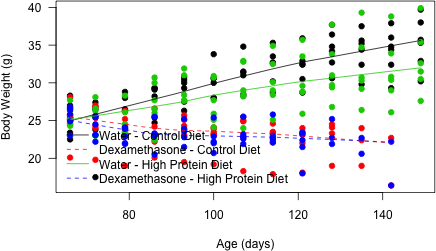
\includegraphics{figures/weights-scatterplot-1.png}
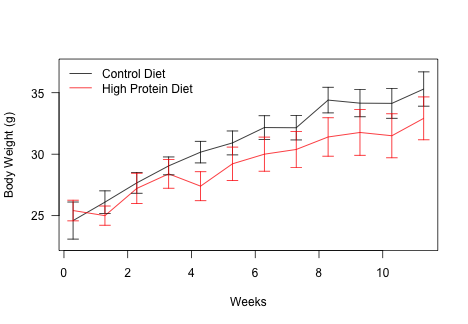
\includegraphics{figures/weights-scatterplot-2.png}

\subsection{Effects of High Protein Diet on Body Weight (Water
Only)}\label{effects-of-high-protein-diet-on-body-weight-water-only}

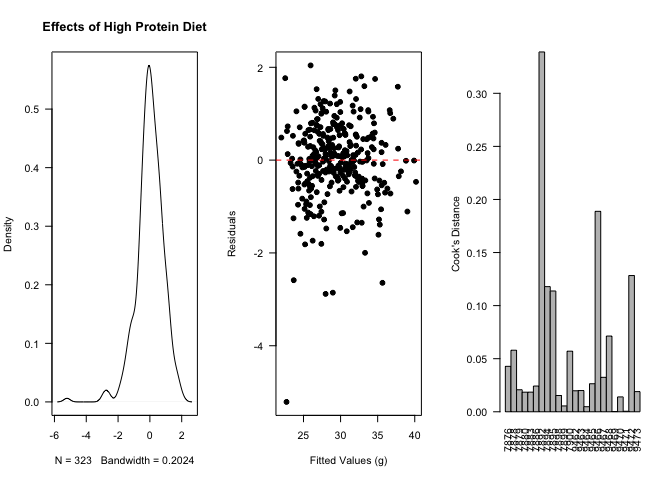
\includegraphics{figures/diagnostics-body-weight-1.png}

Based on linear fixed effects models, allowing for uncorrelated
intercepts and slopes for the animals, within the water group, the High
Protein Diet animals gained -0.26998g weight per week, or -3.23978g over
the experiment. This is a -29.02327\% change in body weight gain. This
effect was significant with a p-value of 0.0368. The residuals of this
model \textbf{did not meet} the presumption of normality via a
Shapiro-Wilk test (p=0).

\subsection{Effects of Dexamethasone on Body Weight (Control Diet
Only)}\label{effects-of-dexamethasone-on-body-weight-control-diet-only}

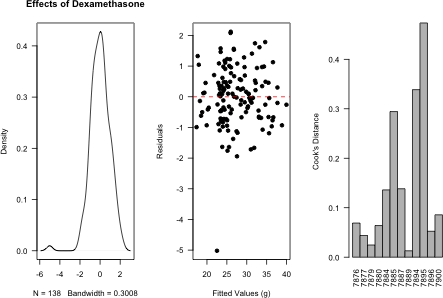
\includegraphics{figures/cooks-distance-dex-1.png}

Based on linear fixed effects models, allowing for uncorrelated
intercepts and slopes for the animals, within the control diet group,
the dexamethasone-treated animals gained -1.15975g weight per week, or
-13.91694g over the experiment. This is a -124.67362\% change in body
weight gain. This effect was significant with a p-value of 0. The
residuals of this model met the presumption of normality via a
Shapiro-Wilk test (p=0.00005).

\section{Combined Analysis}\label{combined-analysis}

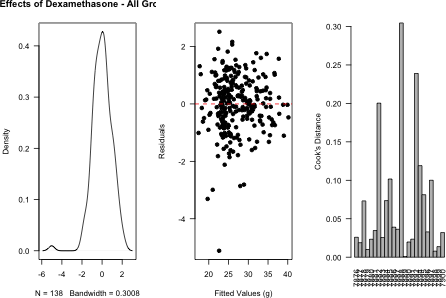
\includegraphics{figures/cooks-distance-combined-1.png}

Pooling both groups together, with a linear fixed effects models,
allowing for uncorrelated intercepts and slopes for the animals, the
dexamethasone-treated animals gained -1.05408g weight per week, or
-12.64902g over the experiment. This is a -119.42968\% change in body
weight gain. This effect was significant with a p-value of 0. The
residuals of this model met the presumption of normality via a
Shapiro-Wilk test (p=0).

\section{Lean Mass}\label{lean-mass}

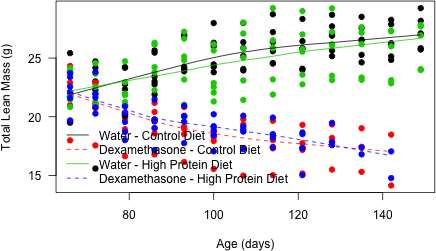
\includegraphics{figures/lean-mass-scatterplot-1.png}
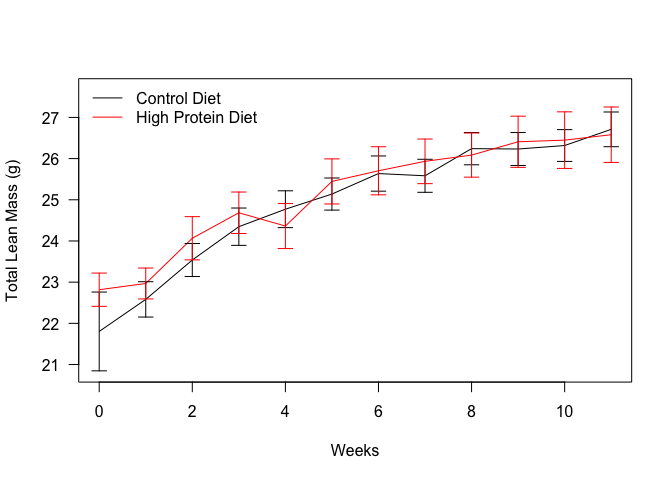
\includegraphics{figures/lean-mass-scatterplot-2.png}

\section{Fat Mass}\label{fat-mass}

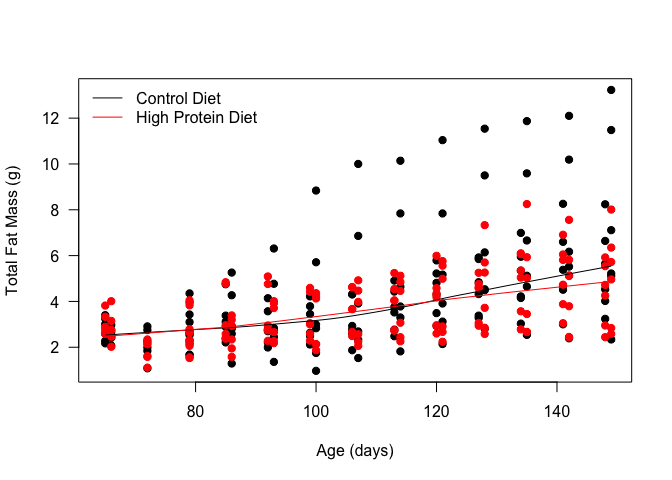
\includegraphics{figures/fat-mass-scatterplot-1.png}
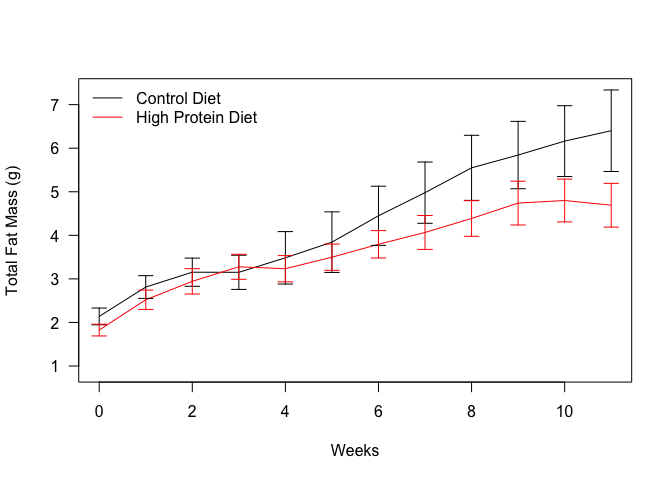
\includegraphics{figures/fat-mass-scatterplot-2.png}

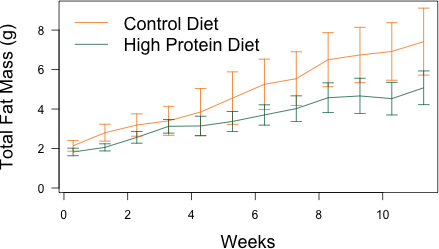
\includegraphics{figures/hpd-fat-mass-scatterplot-uthsc-1.png}

\section{Percent Fat Mass}\label{percent-fat-mass}

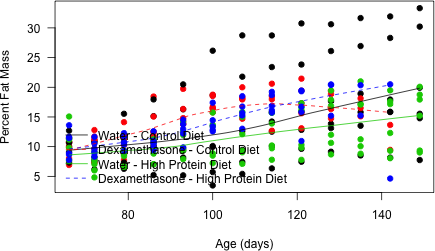
\includegraphics{figures/percent-fat-mass-scatterplot-1.png}

\section{Effects of High Protein Diet
Only}\label{effects-of-high-protein-diet-only}

\subsection{Percent Fat Mass}\label{percent-fat-mass-1}

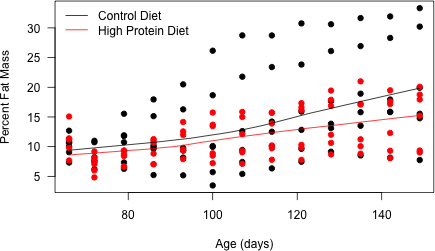
\includegraphics{figures/percent-fat-mass-scatterplot-hpd-1.png}

Based on a mixed linear model with a random slope and intercept for each
animal, there was a significant decrease in the rate of percent fat mass
with respect to time (Chisq = 5.69599, p=0.05796). This as an average
difference of -0.46236 +/- 0.26817 percent fat per week, or a total of
-11.88913 +/- 6.89588 over the course of the study. This is a 44.91657\%
reduction.

\subsection{Total Fat Mass}\label{total-fat-mass}

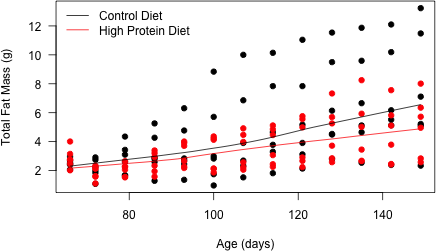
\includegraphics{figures/total-fat-mass-scatterplot-hpd-1.png}

Based on a mixed linear model with a random slope and intercept for each
animal, there was a significant decrease in the rate of percent fat mass
with respect to time (Chisq = 5.74781, p=0.05648). This as an average
difference of -0.21508 +/- 0.12801 percent fat per week, or a total of
-2.36589 +/- 1.40809 over the course of the study. This is a 46.0016\%
reduction.

\section{Session Information}\label{session-information}

\begin{verbatim}
## R version 3.2.2 (2015-08-14)
## Platform: x86_64-apple-darwin13.4.0 (64-bit)
## Running under: OS X 10.10.4 (Yosemite)
## 
## locale:
## [1] en_US.UTF-8/en_US.UTF-8/en_US.UTF-8/C/en_US.UTF-8/en_US.UTF-8
## 
## attached base packages:
## [1] stats     graphics  grDevices utils     datasets  methods   base     
## 
## other attached packages:
## [1] influence.ME_0.9-6 lme4_1.1-8         Matrix_1.2-2      
## [4] tidyr_0.2.0        dplyr_0.4.2        knitr_1.11        
## 
## loaded via a namespace (and not attached):
##  [1] Rcpp_0.12.0     magrittr_1.5    splines_3.2.2   MASS_7.3-43    
##  [5] lattice_0.20-33 R6_2.1.1        minqa_1.2.4     stringr_1.0.0  
##  [9] tools_3.2.2     parallel_3.2.2  grid_3.2.2      nlme_3.1-121   
## [13] DBI_0.3.1       htmltools_0.2.6 yaml_2.1.13     lazyeval_0.1.10
## [17] assertthat_0.1  digest_0.6.8    nloptr_1.0.4    formatR_1.2    
## [21] evaluate_0.7.2  rmarkdown_0.7   stringi_0.5-5
\end{verbatim}

\end{document}
